\section{Summary}

\begin{itemize}
	\item In simulation of queueing systems,
	the center of attention is a simulation entity,
	an object with a state subject to (the actions of) simulation events.
	\item In \lstinline|jqueues|, simulation entities are represented
	as \lstinline|SimEntity| objects.
	In the present release,
	a \lstinline|SimEntity| is either a \lstinline|SimJob|
	(job) or \lstinline|SimQueue| (or their abstract joint interface,
	\lstinline|SimJQ|).
	However, other types of \lstinline|SimEntity| may be added in a future release.
	\item A \lstinline|SimEntity| has the obligation to report
	changes to its state (as a result of event-list processing)
	to registered listeners,
	which are of type \lstinline|SimEntityListener|.
	Listeners to a \lstinline|SimEntity| can be registered and
	unregistered at any time through the
	\lstinline|SimEntity.registerSimEntityListener|
	and \lstinline|SimEntity.unregisterSimEntityListener|
	methods, respectively.
	\item In \lstinline|jqueues|, changes to the state
	of a \lstinline|SimEntity| is always the result
	of the invocation of one of a set of well-defined
	operations on the entity.
	The specific type of \lstinline|SimEntity|
	determines the operation it supports.
	The invocation of an operation is
	almost always performed by a scheduled event.
	\item An operation can be external or internal.
	Events for internal events can only be scheduled
	by the \lstinline|SimEntity| itself.
	\item Upon reception of {\em any\/} operation invocation,
	but before doing anything,
	a \lstinline|SimEntity| fires an \lstinline|UPDATE|
	notification exposing the {\em a priori\/} state
	(i.e., the "old" state).
	\item After completion of an operation invocation,
	but {\em before\/} handing back control (to the event list),
	a \lstinline|SimEntity| fires a \lstinline|STATE CHANGED|
	notification exposing the {\em a posteriori\/} state
	(i.e., the "new" state).
	In some cases, no state-change notification is fired when
	the state did not actually change.
	\item The external operations on a \lstinline|SimQueue| are
	\lstinline|Arrive| and \lstinline|Revoke|.
	\item In \lstinline|jqueues|,
	a \lstinline|SimJob| starts a visit to a \lstinline|SimQueue|
	through the \lstinline|Arrive| operation.
	Listeners are always notified of invocations of \lstinline|Arrive|,
	even if no state change occurs on the entity.
	\item While a \lstinline|SimJob| is present (visiting) a \lstinline|SimQueue|,
	it is either in its waiting or service area.
	Upon arrival, a \lstinline|SimJob| enters the waiting area.
	Moving a \lstinline|SimJob| from the waiting to the service area
	is performed (if at all) through the internal \lstinline|START|
	operation.
	Invocations of the \lstinline|Start| operation are always notified to
	listeners, even if no state change occurs.
	\item The visit of a \lstinline|SimJob| to a \lstinline|SimQueue|
	can end in one of following three ways: (1) Through departure
	(the internal \lstinline|Depart| operation), (2) through dropping
	(the internal \lstinline|Drop| operation), or (3) through revocation
	(the external \lstinline|Revoke| operation or the internal \lstinline|AutoRevoke| operation).
	Whatever way the \lstinline|SimJob| leaves, it can be from the waiting
	and service area.
	Invocations of the \lstinline|Drop| operation are always notified to
	listeners, even if no state change occurs.
	\item A job that is present on a queue, but never leaves during a simulation run
	is named a sticky job.
\end{itemize}

\section{The \texttt{UPDATE} and \texttt{STATE CHANGED} Notifications}

As you may have spotted,
events are actually reported twice,
once as part of a \lstinline|STATE CHANGED| notification,
followed by a separate notification specific to the event type
(\lstinline-ARRIVAL-, \lstinline-DEPARTURE-, etc.).
As a matter of fact, these separate notifications are merely a courtesy
of the queue as it is only required to issue
\lstinline|UPDATE|, \lstinline|STATE CHANGED| and \lstinline|RESET| notifications.

In order to understand this,
  we must realize that in {\em any\/} discrete-event simulation,
  the entities (like queues) involved possess an individual {\em state\/}
  that can only change at discrete moments in time (the {\em epochs\/}),
  and as a result of an {\em operation\/} on the entity at that time.
This is explained graphically in Figure \ref{fig:SimpleSimulationOverview}.

\begin{figure}[h]
	\label{fig:SimpleSimulationOverview}
	\caption{The relations between simulation time, epochs,
		the event list, scheduled events, and actions,
		as well their impact on notifications from
		and operations on
		(the state of) an entity.}
	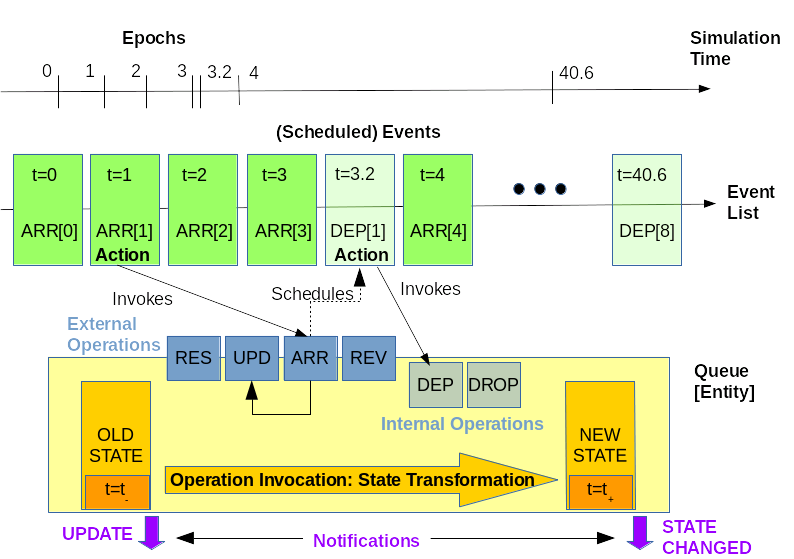
\includegraphics[width=\textwidth]{fig/SimpleSimulationOverview}
\end{figure}

In the top of the figure,
we show the simulation time and some of the epochs
from the example.
During a simulation run, the simulation time increases monotonically
as a function of "real time".
What this says is that the simulation time does not
"strictly decrease" in real time,
but at the same time,
that's pretty much the only requirement
on the relation between real time
and simulation time.
For instance,
processing the epochs between $t=0$ and $t=9$
may take several minutes in real time,
whereas epochs between $t=9$ and $t=100$
could be done in a mere second\footnote{
	This is not to say that is is impossible or even hard
	to let simulation time progress
	(roughly) at the same rate as real time,
	or at some scaled version of it.
	However, in discrete-event simulation,
	the relationship between real time and simulation time
	is generally considered unimportant.}

Below the simulation-time line,
we show the event list and some of the scheduled events
from the example.
The apparent equal distance between the events
is actually on pupose.
The event list is really not concerned with the
simulation-time differences between adjacent events.
No matter how large the time interval between an
event and its predecessor,
in between (basicaly) nothing happened:
There were not events,
and hence,
no state changes.
Going back to the figure,
we scheduled the arrival events ourselves
before processing the event list,
but we also see two "departure events"
we did not schedule.
In fact, these events were scheduled by the
queue, in response to previous events.
For instance, when job $1$ arrives at $t=1$ (simulation time),
it is taken into service immediately,
and after requesting the service time from job $1$ ($2.2$),
it schedules a {\em departure event\/} at $t=3.2$,
shown in a somewhat different color because we
did not schedule this ourselves (we are not even allowed to do so).
This shows an important aspect of the event list while processing it:
in general, the actions taken while processing the event list have
full freedom to schedule new events,
as long as they are not in the past.
This, admittedly, is not clear from the figure.
What is essential to remember is that a scheduled event
await its turn while the event list is being processed,
and the event list invokes the event's action
when it has processed all preceding events.

Assuming the event's action involves the queue in question,
we now turn our attention to the bottom part of the figure,
showing our queue from the example, the \lstinline|FCFS_B| queue.
We assume the arrival event at $t=1$ is processed by the event list,
and the net effect of this (i.e., the action of the event)
is the invokation of the arrival operation on the queue
(with the job $1$ as its argument).
As a result of this operation,
the state of the queue will transform,
and registered listeners to the queue will be informed
of the new state upon completion of the operation.
This, effectively, is the \lstinline|STATE CHANGED| notification.
In the figure this is shown with the right-pointing arrow at the bottom
from \lstinline|OLD STATE| to \lstinline|NEW STATE|,
and the \lstinline|STATE CHANGED| notification below that.

However, before doing anything,
the arrival operation invokes
the so-called \lstinline|UPDATE| operation,
which exposes the {\em old\/} state
to listeners and internally registered "hooks",
and, subsequently, increases the most essential state
property, the {\em last update time}.
By now, you should realize that
as the event list progresses in simulation time,
queues (or better, {\em entities\/})
that are not affected by the events processed
will not be bothered at all.
Yet a queue needs to assure that time-stamped operations
never lie in the past,
so they need to maintain a notion of simulation time themselves.
The importance of the \lstinline|UPDATE| notification
lies in {\em statistics gathering},
in which it is essential to know exactly
during which (non-trivial) intervals
the state of a queue did {\em not\/} change,
and the lenght of such intervals.
As long as you are not involved in statistics-gathering,
you can safely ignore these notifications,
otherwise,
you can find more details in Section \ref{chap:statistics}.

Once the \lstinline|UPDATE| operation has been
fulfilled, the \lstinline|ARR| (job arrival) operation,
in this particular case,
checks the number of jobs waiting,
and drops the arriving job if the number is $2$ ($=$\lstinline|B|)
by invoking the internal operation \lstinline|DROP|.
However, for job $1$ in the example,
it finds an empty waiting area,
and, in addition, no job being served at the server.
This means that the job is taking into service immediately
(the \lstinline|START| internal operation),
and since the required service time is non-zero,
the queue schedules a {\em departure event\/}
at $t=3.2$.
The departur event, in turn,
will invoke the internal \lstinline|DEP| (job departure)
event because of which the job
will eventually depart from the queueing system.

So, what more is there to say.
Well, we seem to have so called {\em external\/}
and {\em internal\/} operations,
the latter of which we cannot schedule ourselves
(departures, drops, $\ldots$).
In a way, the external operations allow us
to subject a queue to some kind of {\em workload\/}
consisting of arriving jobs
(as well as of, yet undescribed, other external operations on the queue).
The internal operations, on the other hand,
are always involved from within the queue itself,
either as a response to a scheduled event,
or as a response to an invocation of an external operation
in combination with a state condition
(e.g., the arrival of a job while $2$ jobs are already waiting
causes the internal \lstinline|DROP| operation to be invoked).

\section{The \texttt{Update} Operation}
\label{sec:guided:update}

In the previous section we introduced the
\lstinline|UPDATE| and \lstinline|STATE CHANGED|
notifications,
and explained that on a \lstinline|SimEntity|,
every state-change must be reported,
and that the \lstinline|UPDATE| notification
exposes the old state of the entity
for (for instance) statistics gathering.
However, there also exits an \lstinline|Update|
operation.
Its function is to set the \lstinline|LastUpdateTime|
state property of the entity.
The example shown in
Listing \ref{simExample1_update_main}
with output
shown in Listing \ref{simExample1_update_out}
demonstrates its use,
again using utility methods
for scheduling.
As the output shows,
there seems to be little use in the \lstinline|Update|
operation; it just updates the time at $t=8.5$ and $t=1000$.
The reason why you would ever want to use \lstinline|Update|
is a bit involved,
and deferred until Chapter \ref{chap:entities-queues-jobs}.
However, we included this example to demonstrate
that the end-time of the simulation can be
controlled through scheduling an \lstinline|Update|
operation.
In the next section, we will delve a little deeper
into the end-time of a simulation.

\begin{lstfloat}
	\begin{lstlisting}[
	caption={The use of the \texttt{Update} operation.},
	label=simExample1_update_main,
	basicstyle=\tiny]
	
	final SimEventList el = new DefaultSimEventList ();
	final int bufferSize = 2;
	final FCFS_B queue = new FCFS_B (el, bufferSize);
	queue.registerStdOutSimEntityListener ();
	for (int j = 0; j < 4; j++)
	{
	final double jobServiceTime = (double) 2.2 * j;
	final double jobArrivalTime = (double) j;
	final String jobName = Integer.toString (j);
	final SimJob job = new DefaultSimJob (null, jobName, jobServiceTime);
	SimJQEventScheduler.scheduleJobArrival (job, queue, jobArrivalTime);
	}
	SimEntityEventScheduler.scheduleUpdate (el, queue, 8.5);
	SimEntityEventScheduler.scheduleUpdate (el, queue, 1000.0);
	el.run ();
	
	\end{lstlisting}
\end{lstfloat}

\begin{lstfloat}
	\begin{lstlisting}[
	caption={The output of Listing \ref{simExample1_update_main}.},
	label=simExample1_update_out,
	basicstyle=\tiny]
	
	StdOutSimEntityListener t=0.0, entity=FCFS_B[2]: UPDATE.
	StdOutSimEntityListener t=0.0, entity=FCFS_B[2]: STATE CHANGED:
	=> ARRIVAL [Arr[0]@FCFS_B[2]]
	=> START [Start[0]@FCFS_B[2]]
	=> DEPARTURE [Dep[0]@FCFS_B[2]]
	StdOutSimEntityListener t=1.0, entity=FCFS_B[2]: UPDATE.
	StdOutSimEntityListener t=1.0, entity=FCFS_B[2]: STATE CHANGED:
	=> ARRIVAL [Arr[1]@FCFS_B[2]]
	=> START [Start[1]@FCFS_B[2]]
	=> STA_FALSE [StartArmed[false]@FCFS_B[2]]
	StdOutSimEntityListener t=2.0, entity=FCFS_B[2]: UPDATE.
	StdOutSimEntityListener t=2.0, entity=FCFS_B[2]: STATE CHANGED:
	=> ARRIVAL [Arr[2]@FCFS_B[2]]
	StdOutSimEntityListener t=3.0, entity=FCFS_B[2]: UPDATE.
	StdOutSimEntityListener t=3.0, entity=FCFS_B[2]: STATE CHANGED:
	=> ARRIVAL [Arr[3]@FCFS_B[2]]
	StdOutSimEntityListener t=3.2, entity=FCFS_B[2]: UPDATE.
	StdOutSimEntityListener t=3.2, entity=FCFS_B[2]: STATE CHANGED:
	=> DEPARTURE [Dep[1]@FCFS_B[2]]
	=> START [Start[2]@FCFS_B[2]]
	StdOutSimEntityListener t=7.6000000000000005, entity=FCFS_B[2]: UPDATE.
	StdOutSimEntityListener t=7.6000000000000005, entity=FCFS_B[2]: STATE CHANGED:
	=> DEPARTURE [Dep[2]@FCFS_B[2]]
	=> START [Start[3]@FCFS_B[2]]
	StdOutSimEntityListener t=8.5, entity=FCFS_B[2]: UPDATE.
	StdOutSimEntityListener t=14.200000000000001, entity=FCFS_B[2]: UPDATE.
	StdOutSimEntityListener t=14.200000000000001, entity=FCFS_B[2]: STATE CHANGED:
	=> DEPARTURE [Dep[3]@FCFS_B[2]]
	=> STA_TRUE [StartArmed[true]@FCFS_B[2]]
	StdOutSimEntityListener t=1000.0, entity=FCFS_B[2]: UPDATE.
	
	\end{lstlisting}
\end{lstfloat}

In summary:
\begin{itemize}
  \item Queues and jobs are collectively referred to as simulation {\em entities}.
  \item Simulation entities always start in a known type-specific {\em default state},
          also referred to their \lstinline|RESET STATE| upon construction
          and upon performing their \lstinline|RESET| operation.
  \item Simulation entities must always report any change to their state through
	  \lstinline|STATE CHANGED| notifications to registered {\em listeners}.
  \item Simulation entities only change their state
          as a result of the invocation of a well-defined
          {\em operation\/} on the entity.
        The operation can be external (like \lstinline-ARRIVAL-)
          or internal (like \lstinline-START-, \lstinline-DROP-, and \lstinline-DEPARTURE-).
  \item Any operation invocation takes zero (simulation) time to perform.
        Upon invocation of an operation, the new simulation time has to be supplied
          by the caller.
        With the exception of the \lstinline|RESET| operation,
          the new time provided must not be strictly smaller than the
          time of the previous invocation (of {\em any\/} operation).
  \item Before even starting the transformation from an old state into a new state,
	  simulation entities must always expose their {\em old\/} state
	  with a \lstinline|UPDATE| notification.
  \item Depending on the registered listener,
	  a simulation entity also fires {\em courtesy\/} notifications,
          revealing only a specific aspect of the state change.
        Courtesy notifications are {\em always\/} fired {\em after\/}
          the applicable \lstinline|STATE CHANGED| notification.
\end{itemize}

\section{Resetting Entities}

Every simulation entity (queue or job) supports the
external \lstinline-RESET- operation
that puts the entity into its {\em default\/} or
{\em reset\/} state.
It is the only operation that is allowed to
set {\em back\/} the time.
The new time on the entity is taken from the event list,
or to $-\infty$ if no event list is available.

The \lstinline-RESET- state of an entity depends
on the type of entity,
but it must be clearly specified.
It is, however, subject to strict rules,
as shown in Tables
\ref{resetStateSettings-queue}
and
\ref{resetStateSettings-job}.
For instance,
in the \lstinline|RESET| state,
a queue is empty (no jobs visiting).
The \lstinline|QueueAccessVacation| and
\lstinline|ServerAccessCredits|
properties will be decribed shortly
in the next sections.
In its \lstinline|RESET| state,
a job is not visiting any queue;
its \lstinline|Queue| propery is \lstinline|null|.
Beware however,
that queues are mandatorily attached to the event list,
whereas for jobs this is not required.
A queue will therefore set
the \lstinline|Queue| property to \lstinline|null|
for the jobs that it forcibly removes.

\begin{table}[h]
	\caption{Mandatory settings in the \texttt{RESET} state
		of a queue.}
	\label{resetStateSettings-queue}
	\begin{center}
		\begin{tabular}{|l|l|l|}
			\hline
			Property & Type & Default Value \\ \hline
			\lstinline|LastUpdateDate|      & \lstinline|double|      & From event list or $-\infty$.               \\ \hline
			\lstinline|Jobs|                & \lstinline|Set<SimJob>| & Empty set.                                  \\ \hline
			\lstinline|QueueAccessVacation| & \lstinline|boolean|     & \lstinline|false|.                          \\ \hline
			\lstinline|ServerAccessCredits| & \lstinline|int|         & \lstinline|Integer.MAX_VALUE| (==$\infty$). \\ \hline
			\lstinline|StartArmed|          & \lstinline|int|         & Depends on \lstinline|SimQueue| type.       \\ \hline
		\end{tabular}
	\end{center}
\end{table}

\begin{table}[h]
	\caption{Mandatory settings in the \texttt{RESET} state
		of a job.}
	\label{resetStateSettings-job}
	\begin{center}
		\begin{tabular}{|l|l|l|}
			\hline
			Property & Type & Default Value \\ \hline
			\lstinline|LastUpdateDate|      & \lstinline|double|      & From event list or $-\infty$.               \\ \hline
			\lstinline|Queue|               & \lstinline|SimQueue|    & \lstinline|null|.                           \\ \hline
		\end{tabular}
	\end{center}
\end{table}

\section{Summary of the \texttt{SimEntity} Interfaces}
\label{sec:guided:simentity-model}

In this section,
having seen almost all aspects of \lstinline|SimEntity|s,
\lstinline|SimJob|s,
and \lstinline|SimQueue|s,
we summarize their state and behavior.
We have two purposes in mind:
\begin{itemize}
	\item To present the material presented thus far in a format
	that allows you to assert your understanding
	of the fundamental concepts in \lstinline|jqueues|
	and \lstinline|jsimulation|.
	\item To present the interfaces in a compact overview format
	that can be used as a reference.
	Really, at this point we have covered almost every aspect
	of entities, queues, and jobs, and their listeners.
	The remainder of this Chapter will focus at some
	left-overs and an important class of queues
	named {\em composite queues}.
	The remainder of this entire book is really
	about explaining rigorously the abstract interfaces
	and the specific concrete types
	of queues (mostly), jobs and listeners,
	and about how you can build your own.
	In other words, the summary presented in this section
	is quite complete already,
	hence it is worth using as a reference.
\end{itemize}







\section{Queue-Access Vacations}
\label{sec:guided:qav}

In \lstinline|jqueues|, every queue,
  in other words, every \lstinline|SimQueue| implementation,
  must support the notion of {\em queue-access vacations}.
During a queue-access vacation,
  {\em all arriving jobs are dropped.}
Butm jobs already visiting the queue are not affected.
In terms of queue state,
  every \lstinline|SimQueue| has a state
  property \lstinline|QueueAccessVacation|
  of type \lstinline|boolean|
  that determines whether or not the
  queue is "on vacation".
The current value of this state property is available through
  \lstinline{SimQueue.isQueueAccessVacation}.
Starting and stoppping queue-access vacations
  is an external operation;
  on any \lstinline{SimQueue} you can
  invoke this operation
  through \lstinline{SimQueue.setQueueAccessVacation(double,boolean)},
  which takes two arguments: (1) the time the operation is invoked,
  and (2), whether the vacation starts of ends.

It is essential to note that queue-access vacations
  are {\em always\/} available to you
  as an independent means to drop ariving jobs
  because you think this is the right thing to do at this time,
  in other words,
  \lstinline|SimQueue| implementations
  are {\em not\/} allowed to use this feature
  in order to get their "jobs done".
This turns the \lstinline|QueueAccessVacation|
  operation into a purely {\em external\/} one.
For instance,
  in our previous example with \lstinline|FCFS_B|,
  the queue {\em could\/} use the mechanism
  of queue-access vacations in order to
  drop jobs upon arrival if the buffer is full.
Yet, it is not allowed to do that.
It simply does not touch the \lstinline|QueueAccessVacation| property.

Scheduling the start and end of queue-access vacations on a queue
  is easily achieved through the utility method
  \lstinline|SimQueueEventScheduler.scheduleQueueAccessVacation (SimQueue, double, boolean)|;
  the respective arguments being the queue to which the event applies,
  the scheduled time,
  and whether or not to start/end a queue-access vacation,
  respectively.
The following example in Listing \ref{simExample3_main}
  show how to schedule a queueu-access vacation from
  $t=1.75$ to $t=2.25$, effectively dropping job $2$
  upon arrival (as its scheduled arrival time is $t=2$).
Our \lstinline|SimQueue| of choice this time is \lstinline|SocPS|.
Just like \lstinline|PS| used in the previous example,
  \lstinline|SocPS| distributes its (full) service capacity
  among the jobs present,
  but, unlike \lstinline|PS|,
  distributes its capacity in such a way that all
  jobs present depart at the same time.
The \lstinline|SocPS| implementation
  is one of our more exotic (maybe even original) ones;
  for more details,
  refer to Section \ref{sec:SocPS}.
Running the code yields the result on \lstinline|System.out|
  as shown in Listing \ref{simExample3_out}.

\begin{lstfloat}
\begin{lstlisting}[
  caption={Setting Queue-Access-Vacations on a \texttt{SocPS} queue.},
  label=simExample3_main,
  basicstyle=\tiny]

    final SimEventList el = new DefaultSimEventList ();
    final SocPS queue = new SocPS (el);
    queue.registerStdOutSimEntityListener ();
    el.reset (1.0);
    SimQueueEventScheduler.scheduleQueueAccessVacation (queue, 1.75, true);
    SimQueueEventScheduler.scheduleQueueAccessVacation (queue, 2.25, false);
    for (int j = 1; j <= 4; j++)
    {
      final double jobServiceTime = (double) 2.2 * j;
      final double jobArrivalTime = (double) j;
      final String jobName = Integer.toString (j);
      final SimJob job = new DefaultSimJob (null, jobName, jobServiceTime);
      SimJQEventScheduler.scheduleJobArrival (job, queue, jobArrivalTime);
    }
    el.run ();

\end{lstlisting}
\end{lstfloat}
  
\begin{lstfloat}
\begin{lstlisting}[
  caption={The output of Listing \ref{simExample3_main}.},
  label=simExample3_out,
  basicstyle=\tiny]

StdOutSimEntityListener t=1.0, entity=SocPS: STATE CHANGED:
  => RESET [Reset@SocPS]
StdOutSimEntityListener entity=SocPS: RESET.
StdOutSimEntityListener t=1.0, entity=SocPS: STATE CHANGED:
  => ARRIVAL [Arr[1]@SocPS]
  => START [Start[1]@SocPS]
StdOutSimEntityListener t=1.75, entity=SocPS: UPDATE.
StdOutSimEntityListener t=1.75, entity=SocPS: STATE CHANGED:
  => QAV_START [QAV[true]@SocPS]
StdOutSimEntityListener t=2.0, entity=SocPS: UPDATE.
StdOutSimEntityListener t=2.0, entity=SocPS: STATE CHANGED:
  => ARRIVAL [Arr[2]@SocPS]
  => DROP [Drop[2]@SocPS]
StdOutSimEntityListener t=2.25, entity=SocPS: UPDATE.
StdOutSimEntityListener t=2.25, entity=SocPS: STATE CHANGED:
  => QAV_END [QAV[false]@SocPS]
StdOutSimEntityListener t=3.0, entity=SocPS: UPDATE.
StdOutSimEntityListener t=3.0, entity=SocPS: STATE CHANGED:
  => ARRIVAL [Arr[3]@SocPS]
  => START [Start[3]@SocPS]
StdOutSimEntityListener t=4.0, entity=SocPS: UPDATE.
StdOutSimEntityListener t=4.0, entity=SocPS: STATE CHANGED:
  => ARRIVAL [Arr[4]@SocPS]
  => START [Start[4]@SocPS]
StdOutSimEntityListener t=18.6, entity=SocPS: UPDATE.
StdOutSimEntityListener t=18.6, entity=SocPS: STATE CHANGED:
  => DEPARTURE [Dep[1]@SocPS]
  => DEPARTURE [Dep[3]@SocPS]
  => DEPARTURE [Dep[4]@SocPS]

\end{lstlisting}
\end{lstfloat}

Indeed, as expected, job $2$ is dropped due to the scheduled queue-access vacation
  upon its arrival.
Despite this,
  the arriving job $3$ still finds job $1$ being (exclusively) served,
  so \lstinline|SocPS| schedules their mutual departure.
However,
  the arrival of job $4$ is ahead of this scheduled departure,
  so \lstinline|SocPS| needs to reschedule the departure time
  (of all jobs present).
Since the total "amount of work"
  of jobs $1$, $3$, and $4$ jointly is $2.2 + 6.6 + 8.8 = 17.6$,
  and the arrival time of job $1$ is $1.0$,
  the joint departure time of jobs $1$, $3$, and $4$,
  should be $1.0+17.6=18.6$,
  which is indeed confirmed in the output.

\section{The Waiting and Service Area of a \texttt{SimQueue}}
\label{sec:guided:wait-serv-area}

Every queue (\lstinline|SimQueue|) consists of
  a {\em waiting area\/} and a {\em service area},
  and visiting jobs are always present in precisely
  one of them,
  see Figure \ref{fig:WaitingAndServiceArea}.
Upon arrival, jobs enter the waiting area.
If they \lstinline|START|,
  they leave the waiting area and
  enter the service area.
An important and perhaps non-intuitive restriction
  is that {\em jobs cannot move back from the service area
  into the waiting area}.
Jobs may \lstinline|DEPART| from,
  be \lstinline|DROP|ped from,
  or be \lstinline|REVOKE|d from
  either area.
Jobs that do {\em not\/} leave the queue
  are named {\em sticky\/} jobs;
  they may reside in either area.

\begin{figure}[h]
\label{fig:WaitingAndServiceArea}
\caption{The waiting and service areas of a \texttt{SimQueue}.}
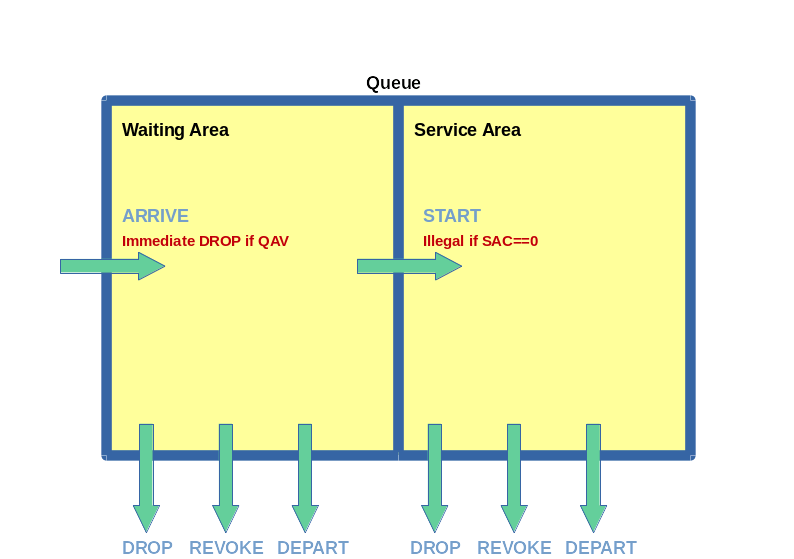
\includegraphics[width=\textwidth]{fig/WaitingAndServiceArea}
\end{figure}

The model for queues in terms of waiting and service area is,
  admittedly, somewhat deviant from models in literature.
The main point is that we make {\em no\/} assumptions
  whatsoever on the structure of the waiting and service areas.
But for most known queueing systems,
  the waiting area is simply a queue holding waiting jobs,
  often in FIFO (First-In First-Out) order,
  and the service area consists of one of more servers
  serving jobs until completion.
In (classical) processor-sharing queues,
  there is virtually no waiting area,
  as jobs enter the service area immediately.

There are two more "complications" to bear in mind:
\begin{itemize}
  \item Since jobs cannot move back from the service area
          into the waiting area,
          one has to let go of the intuitive notion that
          jobs in the service area area actually {\em being served}.
        Despite the fact that this is true for many queueing systems,
          it is false for systems like Preemptive/Resume Last-Come First-Served
          (\lstinline|P_LCFS|),
          and many other preemptive queueing systems.
        In \lstinline|P_LCFS|, whenever a job in the service area is preempted
          in favor of a new arrival,
          the preempted jobs stays in the service area,
          yet receives no service (at least, not for a while).
  \item In order for jobs to be eligible to \lstinline|START|,
          the queue needs so-called \lstinline|ServerAccessCredits|.
        These are described in more detail in the next section.
\end{itemize}

In Table \ref{simqueue-methods-areas},
  we list the most important methods related to waiting and service areas
  on a \lstinline|SimQueue|.

\begin{table}[h]
\caption{\texttt{SimQueue} methods related to waiting and service areas.}
\label{simqueue-methods-areas}
\begin{center}
\begin{tabular}{|l|l|l|}
\hline
Prototype & Symbol & Remark \\ \hline
\lstinline|getJobs|                      & $J(t)$      & The jobs visiting the \lstinline|SimQueue|.       \\ \hline
\lstinline|getNumberOfJobs|              & $|J(t)|$    & The number of jobs currently visiting.            \\ \hline
\lstinline|isJob (SimJob)|               &             & Checks presence of given job.                     \\ \hline
\lstinline|getJobsInWaitingArea|         & $J_w(t)$    & The jobs in the waiting area.                     \\ \hline
\lstinline|getNumberOfJobsInWaitingArea| & $|J_w(t)|$  & The number of jobs in the waiting area.           \\ \hline
\lstinline|isJobInWaitingArea (SimJob)|  &             & Checks presence of given job in the waiting area. \\ \hline
\lstinline|getJobsInServiceArea|         & $J_s(t)$    & The jobs in the service area.                     \\ \hline
\lstinline|getNumberOfJobsInServiceArea| & $|J_s(t)|$  & The number of jobs in the service area.           \\ \hline
\lstinline|isJobInServiceArea (SimJob)|  &             & Checks presence of given job in the service area. \\ \hline
\end{tabular}
\end{center}
\end{table}

\section{Server-Access Credits}
\label{sec:guided:sac}

The \lstinline|ServerAccessCredits|
  is a state property on every \lstinline|SimQueue|,
  and setting its value is an
  external operation
  named \lstinline|SetServerAccessCredits|.
Its value represents the maximum number of
  jobs on that particular \lstinline|SimQueue|
  that can \lstinline|START|,
  in other words,
  move from the waiting area into
  the service area;
  see also Figure \ref{fig:WaitingAndServiceArea}.
Whenever a job starts,
  the \lstinline|ServerAccessCredits| value
  is decremented with one,
  and if it reaches zero,
  jobs are no longer allowed to start.
The \lstinline|ServerAccessCredits| value
  {\em never\/}
  affects jobs that are already in the
  service area.

Every \lstinline|SimQueue| reports
  changes to {\em the availability of server-access credits\/}
  (i.e., not just changes to the actual value)
  through the \lstinline|LOST_SAC|
  and \lstinline|REGAINED SAC|
  notification.
The former notification can be the result of
  starting one or more jobs
  {\em or\/}
  the invocation of \lstinline|SetServerAccessCredits|
  with argument zero,
  whereas the latter notification is always
  the result of \lstinline|SetServerAccessCredits|
  with argument (at least) non-zero.

Since the server-access credits are an integral number,
  it is represented by \lstinline|Java|'s
  \lstinline|int| simple type,
  but the value
  \lstinline|Integer.MAX_VALUE|
  is interpreted as infinity.
This is in fact the default value,
  as can be see in Table \ref{resetStateSettings-queue},
  and as long as \lstinline|ServerAccessCredits|
  has this value,
  it is not affected by starting jobs
  (the value is not decremented),
  effectively turning off the mechanism of
  server-access credits.

In addition to the default value being $\infty$,
  \lstinline|SimQueue| implementations
  cannot use \lstinline|ServerAccessCredits|
  to meet their requirements.
For instance, in order to implement queueing
  systems with multiple servers like
  \lstinline|FCFS_c|
  (see Section \ref{sec:FCFS_c}),
  the use of
  \lstinline|ServerAccessCredits|
  could be queue handy.
However, decrementing the value upon \lstinline|START|
  of a job is the only thing queues may do
  (and must adhere to).

These two facts imply that
  if you never "touch"
  the \lstinline|ServerAccessCredits|
  through the use of
  \lstinline|SetServerAccessCredits|,
  you can safely forget the entire concept.
On the other hand,
  should you have any need for it,
  it is always available,
  whatever the (concrete) queue type.

For our example showing the use of server-access credits,
  shown in Listing \ref{simExample4_main},
  we switch queues again,
  and select a \lstinline|FCFS_c| queue.
In the example, after creating the queue
  and resetting the event list,
  we schedule (!) setting the server-access credits
  on the queue to zero at $t=0$,
  again using a utility method
  from \lstinline|SimQueueEventScheduler|.
We then schedule six jobs
  with one second inter-arrival time
  starting at $t=1$,
  each requiring $1.05$ service time.
Finally we schedule setting the server-access credits
  to unity at $t=8$,
  to three at $t=10$,
  and to infinity at $t=15$.
We show the output of the program in
  Listing \ref{simExample4_out}.

\begin{lstfloat}
\begin{lstlisting}[
  caption={Setting Server-Access Credits on a \texttt{FCFS\_c} queue.},
  label=simExample4_main,
  basicstyle=\tiny]

    final SimEventList el = new DefaultSimEventList ();
    final FCFS_c queue = new FCFS_c (el, 2);
    queue.registerStdOutSimEntityListener ();
    el.reset (0.0);
    SimQueueEventScheduler.scheduleServerAccessCredits (queue, 0.0, 0);
    for (int j = 1; j <= 6; j++)
    {
      final double jobServiceTime = 1.05;
      final double jobArrivalTime = (double) j;
      final String jobName = Integer.toString (j);
      final SimJob job = new DefaultSimJob (null, jobName, jobServiceTime);
      SimJQEventScheduler.scheduleJobArrival (job, queue, jobArrivalTime);
    }
    SimQueueEventScheduler.scheduleServerAccessCredits (queue,  8.0, 1);
    SimQueueEventScheduler.scheduleServerAccessCredits (queue, 10.0, 3);
    SimQueueEventScheduler.scheduleServerAccessCredits (queue, 15.0, Integer.MAX_VALUE);
    el.run ();

\end{lstlisting}
\end{lstfloat}
  
\begin{lstfloat}
\begin{lstlisting}[
  caption={The output of Listing \ref{simExample4_main}.},
  label=simExample4_out,
  basicstyle=\tiny]

StdOutSimEntityListener t=0.0, entity=FCFS_2: STATE CHANGED:
  => RESET [Reset@FCFS_2]
StdOutSimEntityListener entity=FCFS_2: RESET.
StdOutSimEntityListener t=0.0, entity=FCFS_2: STATE CHANGED:
  => OUT_OF_SAC [SAC[0]@FCFS_2]
StdOutSimEntityListener t=1.0, entity=FCFS_2: UPDATE.
StdOutSimEntityListener t=1.0, entity=FCFS_2: STATE CHANGED:
  => ARRIVAL [Arr[1]@FCFS_2]
StdOutSimEntityListener t=2.0, entity=FCFS_2: UPDATE.
StdOutSimEntityListener t=2.0, entity=FCFS_2: STATE CHANGED:
  => ARRIVAL [Arr[2]@FCFS_2]
StdOutSimEntityListener t=3.0, entity=FCFS_2: UPDATE.
StdOutSimEntityListener t=3.0, entity=FCFS_2: STATE CHANGED:
  => ARRIVAL [Arr[3]@FCFS_2]
StdOutSimEntityListener t=4.0, entity=FCFS_2: UPDATE.
StdOutSimEntityListener t=4.0, entity=FCFS_2: STATE CHANGED:
  => ARRIVAL [Arr[4]@FCFS_2]
StdOutSimEntityListener t=5.0, entity=FCFS_2: UPDATE.
StdOutSimEntityListener t=5.0, entity=FCFS_2: STATE CHANGED:
  => ARRIVAL [Arr[5]@FCFS_2]
StdOutSimEntityListener t=6.0, entity=FCFS_2: UPDATE.
StdOutSimEntityListener t=6.0, entity=FCFS_2: STATE CHANGED:
  => ARRIVAL [Arr[6]@FCFS_2]
StdOutSimEntityListener t=8.0, entity=FCFS_2: UPDATE.
StdOutSimEntityListener t=8.0, entity=FCFS_2: STATE CHANGED:
  => START [Start[1]@FCFS_2]
StdOutSimEntityListener t=9.05, entity=FCFS_2: UPDATE.
StdOutSimEntityListener t=9.05, entity=FCFS_2: STATE CHANGED:
  => DEPARTURE [Dep[1]@FCFS_2]
StdOutSimEntityListener t=10.0, entity=FCFS_2: UPDATE.
StdOutSimEntityListener t=10.0, entity=FCFS_2: STATE CHANGED:
  => START [Start[2]@FCFS_2]
  => START [Start[3]@FCFS_2]
  => REGAIN_SAC [SAC[1]@FCFS_2]
  => STA_FALSE [StartArmed[false]@FCFS_2]
StdOutSimEntityListener t=11.05, entity=FCFS_2: UPDATE.
StdOutSimEntityListener t=11.05, entity=FCFS_2: STATE CHANGED:
  => DEPARTURE [Dep[2]@FCFS_2]
  => START [Start[4]@FCFS_2]
  => OUT_OF_SAC [SAC[0]@FCFS_2]
StdOutSimEntityListener t=11.05, entity=FCFS_2: STATE CHANGED:
  => DEPARTURE [Dep[3]@FCFS_2]
  => STA_TRUE [StartArmed[true]@FCFS_2]
StdOutSimEntityListener t=12.100000000000001, entity=FCFS_2: UPDATE.
StdOutSimEntityListener t=12.100000000000001, entity=FCFS_2: STATE CHANGED:
  => DEPARTURE [Dep[4]@FCFS_2]
StdOutSimEntityListener t=15.0, entity=FCFS_2: UPDATE.
StdOutSimEntityListener t=15.0, entity=FCFS_2: STATE CHANGED:
  => START [Start[5]@FCFS_2]
  => START [Start[6]@FCFS_2]
  => REGAIN_SAC [SAC[2147483647]@FCFS_2]
  => STA_FALSE [StartArmed[false]@FCFS_2]
StdOutSimEntityListener t=16.05, entity=FCFS_2: UPDATE.
StdOutSimEntityListener t=16.05, entity=FCFS_2: STATE CHANGED:
  => DEPARTURE [Dep[5]@FCFS_2]
  => STA_TRUE [StartArmed[true]@FCFS_2]
StdOutSimEntityListener t=16.05, entity=FCFS_2: STATE CHANGED:
  => DEPARTURE [Dep[6]@FCFS_2]

\end{lstlisting}
\end{lstfloat}

The output shows indeed that at $t=0$,
  the queue fires a notification \lstinline|OUT_OF_SAC|.
This makes sense, since the server-access credits
  were set to zero from their default
  value infinity.
Subsequently,
  the arrival of the jobs at $t=1, 2, \ldots$,
  is reported,
  but since there are no server-access credits,
  the jobs cannot start.
The behavior of \lstinline|FCFS_c|
  (and many other queueing systems)
  to maintain arrival-time ordering
  of the jobs in the waiting area,
  irrespective of
  whether these jobs are waiting for
  server-access credits or server availability.
At $t=8$, the queue is given a single
  server-access credit,
  and it immediately uses it to
  take job $1$ into service.
What we want to emphasize is that
  despite the server-access credit given to the queue,
  the queue does {\em not\/} issue a notification
  that it has regained server-access credits,
  because the credit is used immediately to start
  job $1$, thus leaving zero credits available;
  the same as the number available before
  invocation of the operation \lstinline|SetServerAccessCredits|
  at $t=8$.
This is a clear example of the {\em atomicity\/}
  of operations and notifications,
  which we shall explain in more detail in Section \ref{sec:guided:atomicity}.
At $t=10$, the queue is granted three additional server-access credits,
  but it can only start two jobs, since it has only two servers available.
Hence, one credit remains after starting the two jobs,
  and this time,
  the queue {\em does\/} issue
  a \lstinline|REGAIN_SAC| notification.
Note that in this particular case,
  the fact that \lstinline|FCFS_c|
  only allows as many jobs in the service area as there are server available,
  is a policy choice of \lstinline|FCFS_c|.
It would have been legal for the queueing system
  to try to move as many jobs are possible from the waiting area
  to the service area upon having been granted new service access credits.
But the choice made in \lstinline|FCFS_c| makes a lot of sense;
  now the \lstinline|START| notification
  is issued the moment a job actually starts its service at a
  server,
  instead of at the otherwise meaningless moment
  of entering the service area
  where is may still have to wait for a server to become available.
The remainder of the notifications are quite trivial.
It should, however,
  be clear that queueing systems have to properly
  specify their behavior in the presence of limited
  server-access credits.
  
\section{Revocations}
\label{sec:guided:revocations}

Up to now,
we have seen two means by which a \lstinline|SimJob|
can end its visit to a \lstinline|SimQueue|:
Through {\em departure\/}
and through {\em drop}.
We also found that jobs may not leave the queue at all;
the sticky jobs.
The final way in which a visit can end is through {\em revocation};
a revocation is a user-initiated exit of a job at a queue.

There are two flavors of revocations:
\begin{itemize}
	\item
	Users can invoke the external \lstinline|REVOKE| operation,
	requesting for the forced exit of a jobs.
	Every \lstinline|SimQueue| must support the operation.
	\item
	Users can set one or more conditions on a queue.
	Once these conditions are met, the queue automatically
	revokes the job.
	Such revocations are named {\em auto-revocations}.
\end{itemize}

We shall discuss each of these flavors in turn.

\subsection{The \texttt{Revoke} Operation}

The external \lstinline|Revoke| operation
{\em requests\/} the removal of a job visiting a queue.
If successful,
a \lstinline|REVOCATION| notification is fired.
On every \lstinline|SimQueue|,
the method \lstinline|revoke (double, SimJob)|
revokes a job unconditionally from the queue.
The first argument is (as always)
the time of the request.
If the job is present a priori,
the revocation request cannot fail;
every \lstinline|SimQueue| implementation
must honor it.
A variant method exists: \lstinline|revoke (double, SimJob, boolean)|,
in which the third argument indicates
whether it is allowed to revoke the job
from the {\em service area}.
If the argument is \lstinline|false| and the job is indeed
in the service area,
the request will fail,
and no notification will be fired.
If, however, the job is in the waiting area,
and/or the argument is set to \lstinline|true|
and the job is present in either area,
then, again, the request cannot fail.

In our example shown in Listing \ref{simExample5_revocations_main}
we use yet another standard queue, Shortest Job First,
or \lstinline|SJF|, a single-server
queueing discipline that selects
the jobs with the shortest required service time
for service when the server becomes idle
(but, it {\em preempts\/} the job currently being served).
In \lstinline|jqueues|,
we have to add the additional requirement
that there are service-access credits available,
as pointed out in Section \ref{sec:guided:sac}.
In the example,
we set the server-access credits to zero at $t=0$,
then we schedule four jobs (at
$t=1, 2, 3, 4$) with service time
$12$, $6$, $4$, and $3$, respectively,
and release all constraints on server-access
credits at $t=10$,
at which time \lstinline|SJF| will
take job $4$ into service because it has the (strictly) smallest
required service time.
The output is shown in Listing \ref{simExample5_revocations_out}.
Of the next two scheduled revocations requests for job $4$,
at $t=11$ and $t=12$, respectively,
the first one will fail because it does not allow
the revocation from the service area,
which is where job$4$ is in at the time of the request.
The second request, though, succeeds, since it allows the
revocation to take place from the service area.
The outcome of the remainder of the scheduled revocation events
is quite trivial.
One thing to bear in mind, though,
is that {\em failed\/} revocation requests mostly
do {\em not\/} lead to a notification;
they just pass by unnoticed
(see for instance the failed revocation attempt
of job $4$ at $t=11$).

\begin{lstfloat}
	\begin{lstlisting}[
	caption={Revocation attempts from a \texttt{SJF} queue.},
	label=simExample5_revocations_main,
	basicstyle=\tiny]
	
	final SimEventList el = new DefaultSimEventList ();
	final SJF queue = new SJF (el);
	queue.registerStdOutSimEntityListener ();
	el.reset (0.0);
	final List<SimJob> jobs = new ArrayList<>  ();
	// Do not allow jobs to start until t=10.
	SimQueueEventScheduler.scheduleServerAccessCredits (queue, 0.0, 0);
	for (int j = 1; j <= 4; j++)
	{
	final double jobServiceTime = 12.0 / j;
	final double jobArrivalTime = (double) j;
	final String jobName = Integer.toString (j);
	final SimJob job = new DefaultSimJob (null, jobName, jobServiceTime);
	jobs.add (job);
	SimJQEventScheduler.scheduleJobArrival (job, queue, jobArrivalTime);
	}
	// Allow jobs to start at t=10.
	SimQueueEventScheduler.scheduleServerAccessCredits (queue, 10.0, Integer.MAX_VALUE);
	// At t=10, the SJF will select job 4 for service since it has the shortest service time (3.0).
	// The next revocation attempt will therefore fail, because job 4 (index 3) is in service,
	// and we do not allow the revocation from the service area.
	SimJQEventScheduler.scheduleJobRevocation (jobs.get (3), queue, 11.0, false);
	// But this attempt will succeed, because this time we allow interruption of service.
	SimJQEventScheduler.scheduleJobRevocation (jobs.get (3), queue, 12.0, true);
	// Because at t=12, job 4 (index 3) is revoked, the queue will take
	// job 3 (index 2) into service, with service time 4.0.
	// This attempt will succeed; job 1 (index 0) is in the waiting queue.
	SimJQEventScheduler.scheduleJobRevocation (jobs.get (0), queue, 13.0, false);
	// However, the next attempt will fail (silently) because job 4 (index 3)
	// is not longer present..
	SimJQEventScheduler.scheduleJobRevocation (jobs.get (3), queue, 15.0, true);
	el.run ();
	
	\end{lstlisting}
\end{lstfloat}

\begin{lstfloat}
	\begin{lstlisting}[
	caption={The output of Listing \ref{simExample5_revocations_main}.},
	label=simExample5_revocations_out,
	basicstyle=\tiny]
	
	StdOutSimEntityListener t=0.0, entity=SJF: STATE CHANGED:
	=> RESET [Reset@SJF]
	StdOutSimEntityListener entity=SJF: RESET.
	StdOutSimEntityListener t=0.0, entity=SJF: STATE CHANGED:
	=> OUT_OF_SAC [SAC[0]@SJF]
	StdOutSimEntityListener t=1.0, entity=SJF: UPDATE.
	StdOutSimEntityListener t=1.0, entity=SJF: STATE CHANGED:
	=> ARRIVAL [Arr[1]@SJF]
	StdOutSimEntityListener t=2.0, entity=SJF: UPDATE.
	StdOutSimEntityListener t=2.0, entity=SJF: STATE CHANGED:
	=> ARRIVAL [Arr[2]@SJF]
	StdOutSimEntityListener t=3.0, entity=SJF: UPDATE.
	StdOutSimEntityListener t=3.0, entity=SJF: STATE CHANGED:
	=> ARRIVAL [Arr[3]@SJF]
	StdOutSimEntityListener t=4.0, entity=SJF: UPDATE.
	StdOutSimEntityListener t=4.0, entity=SJF: STATE CHANGED:
	=> ARRIVAL [Arr[4]@SJF]
	StdOutSimEntityListener t=10.0, entity=SJF: UPDATE.
	StdOutSimEntityListener t=10.0, entity=SJF: STATE CHANGED:
	=> START [Start[4]@SJF]
	=> REGAIN_SAC [SAC[2147483647]@SJF]
	=> STA_FALSE [StartArmed[false]@SJF]
	StdOutSimEntityListener t=12.0, entity=SJF: UPDATE.
	StdOutSimEntityListener t=12.0, entity=SJF: STATE CHANGED:
	=> REVOCATION [Rev[4]@SJF]
	=> START [Start[3]@SJF]
	StdOutSimEntityListener t=13.0, entity=SJF: UPDATE.
	StdOutSimEntityListener t=13.0, entity=SJF: STATE CHANGED:
	=> REVOCATION [Rev[1]@SJF]
	StdOutSimEntityListener t=16.0, entity=SJF: UPDATE.
	StdOutSimEntityListener t=16.0, entity=SJF: STATE CHANGED:
	=> DEPARTURE [Dep[3]@SJF]
	=> START [Start[2]@SJF]
	StdOutSimEntityListener t=22.0, entity=SJF: UPDATE.
	StdOutSimEntityListener t=22.0, entity=SJF: STATE CHANGED:
	=> DEPARTURE [Dep[2]@SJF]
	=> STA_TRUE [StartArmed[true]@SJF]
	
	\end{lstlisting}
\end{lstfloat}

\subsection{Auto-Revocations}

Auto-revocations are forced removals from a \lstinline|SimQueue|
because a user-set condition is met.
The set of conditions for auto-revocation
that can be set on a \lstinline|SimQueue|
depends on the queue's type,
however,
every \lstinline|SimQueue|
must have {\em any\/}
auto-revocation condition
{\em disabled by default}.
The only auto-revocation condition
every \lstinline|SimQueue| {\em must\/}
support, is the start of a job.
(But, it must be disabled by default.)
A simple example of this feature is given
in Listings \ref{simExample5_autorevocations_main}
and \ref{simExample5_autorevocations_out},
again using the \lstinline|SJF|
queueing system.
Note that successful auto-revocations
yield a special notification,
\lstinline|AUTO_REVOCATION|.

\begin{lstfloat}
	\begin{lstlisting}[
	caption={Auto-revocations from a \texttt{SJF} queue.},
	label=simExample5_autorevocations_main,
	basicstyle=\tiny]
	
	final SimEventList el = new DefaultSimEventList ();
	final SJF queue = new SJF (el);
	queue.registerStdOutSimEntityListener ();
	// Set auto-revocation upon start.
	queue.setAutoRevocationPolicy (SimQueue.AutoRevocationPolicy.UPON_START);
	el.reset (0.0);
	final List<SimJob> jobs = new ArrayList<>  ();
	// Do not allow jobs to start until t=10.
	SimQueueEventScheduler.scheduleServerAccessCredits (queue, 0.0, 0);
	for (int j = 1; j <= 4; j++)
	{
	final double jobServiceTime = 12.0 / j;
	final double jobArrivalTime = (double) j;
	final String jobName = Integer.toString (j);
	final SimJob job = new DefaultSimJob (null, jobName, jobServiceTime);
	jobs.add (job);
	SimJQEventScheduler.scheduleJobArrival (job, queue, jobArrivalTime);
	}
	// Allow two jobs to start at t=10.
	// These will be immediately auto-revoked.
	SimQueueEventScheduler.scheduleServerAccessCredits (queue, 10.0, 2);
	// Allow the other two jobs to start at t=13.
	// These, again, will be immediately auto-revoked.
	SimQueueEventScheduler.scheduleServerAccessCredits (queue, 13.0, Integer.MAX_VALUE);    
	el.run ();
	
	\end{lstlisting}
\end{lstfloat}

\begin{lstfloat}  
	\begin{lstlisting}[
	caption={The output of Listing \ref{simExample5_autorevocations_main}.},
	label=simExample5_autorevocations_out,
	basicstyle=\tiny]
	
	StdOutSimEntityListener t=0.0, entity=SJF: STATE CHANGED:
	=> RESET [Reset@SJF]
	StdOutSimEntityListener entity=SJF: RESET.
	StdOutSimEntityListener t=0.0, entity=SJF: STATE CHANGED:
	=> OUT_OF_SAC [SAC[0]@SJF]
	StdOutSimEntityListener t=1.0, entity=SJF: UPDATE.
	StdOutSimEntityListener t=1.0, entity=SJF: STATE CHANGED:
	=> ARRIVAL [Arr[1]@SJF]
	StdOutSimEntityListener t=2.0, entity=SJF: UPDATE.
	StdOutSimEntityListener t=2.0, entity=SJF: STATE CHANGED:
	=> ARRIVAL [Arr[2]@SJF]
	StdOutSimEntityListener t=3.0, entity=SJF: UPDATE.
	StdOutSimEntityListener t=3.0, entity=SJF: STATE CHANGED:
	=> ARRIVAL [Arr[3]@SJF]
	StdOutSimEntityListener t=4.0, entity=SJF: UPDATE.
	StdOutSimEntityListener t=4.0, entity=SJF: STATE CHANGED:
	=> ARRIVAL [Arr[4]@SJF]
	StdOutSimEntityListener t=10.0, entity=SJF: UPDATE.
	StdOutSimEntityListener t=10.0, entity=SJF: STATE CHANGED:
	=> START [Start[4]@SJF]
	=> AUTO_REVOCATION [AutoRev[4]@SJF]
	=> START [Start[3]@SJF]
	=> AUTO_REVOCATION [AutoRev[3]@SJF]
	StdOutSimEntityListener t=13.0, entity=SJF: UPDATE.
	StdOutSimEntityListener t=13.0, entity=SJF: STATE CHANGED:
	=> START [Start[2]@SJF]
	=> AUTO_REVOCATION [AutoRev[2]@SJF]
	=> START [Start[1]@SJF]
	=> AUTO_REVOCATION [AutoRev[1]@SJF]
	=> REGAIN_SAC [SAC[2147483647]@SJF]
	
	\end{lstlisting}
\end{lstfloat}

\subsection{Notification Types}

In Table \ref{tab:guided:notification-types},
we summarize the notification types supported on a \lstinline|SimQueue|,
subdivided into \lstinline|SimEntity|, \lstinline|SimJQ|
and \lstinline|SimQueue| notification types.
The \lstinline|SimEntity| notification types
apply to any \lstinline|SimEntity|,
the \lstinline|SimJQ| types to \lstinline|SimJob|s and \lstinline|SimQueue|s,
and the \lstinline|SimQueue| types to \lstinline|SimQueue|s only.

\begin{table}
	\label{tab:guided:notification-types}
	\caption{The notification types from a \texttt{SimQueue}.}
	\begin{center}
		\begin{longtabu}{|l|l|}
			\hline
			\multicolumn{2}{|c|}{} \\
			\multicolumn{2}{|c|}{\lstinline[basicstyle=\ttfamily]{SimEntity} Notification Types} \\
			\multicolumn{2}{|c|}{} \\
			\hline
			\lstinline|RESET|         & \lstinline|double newTime|                                                \\ \hline
			\lstinline|UPDATE|        & \lstinline|double oldTime|                                                \\ \hline
			\lstinline|STATE CHANGED| & \lstinline|double time|, \lstinline|Set<SimEntityEvent> subNotifications| \\ \hline
			\hline
			\multicolumn{2}{|c|}{} \\
			\multicolumn{2}{|c|}{\lstinline[basicstyle=\ttfamily]{SimJQ} Notification Types} \\
			\multicolumn{2}{|c|}{} \\
			\hline
			\lstinline|ARRIVAL|            & \lstinline|double time|, \lstinline|SimJob|, \lstinline|SimQueue| \\ \hline
			\lstinline|DROP|               & \lstinline|double time|, \lstinline|SimJob|, \lstinline|SimQueue| \\ \hline
			\lstinline|REVOCATION|         & \lstinline|double time|, \lstinline|SimJob|, \lstinline|SimQueue| \\ \hline
			\lstinline|AUTO_REVOCATION|    & \lstinline|double time|, \lstinline|SimJob|, \lstinline|SimQueue| \\ \hline
			\lstinline|START|              & \lstinline|double time|, \lstinline|SimJob|, \lstinline|SimQueue| \\ \hline
			\lstinline|DEPARTURE|          & \lstinline|double time|, \lstinline|SimJob|, \lstinline|SimQueue| \\ \hline
			\hline
			\multicolumn{2}{|c|}{} \\
			\multicolumn{2}{|c|}{\lstinline[basicstyle=\ttfamily]{SimQueue} Notification Types} \\
			\multicolumn{2}{|c|}{} \\
			\hline
			\lstinline|QAV_START|    & \lstinline|double time|, \lstinline|SimQueue| \\ \hline
			\lstinline|QAV_END|      & \lstinline|double time|, \lstinline|SimQueue| \\ \hline
			\lstinline|OUT_OF_SAC|   & \lstinline|double time|, \lstinline|SimQueue| \\ \hline
			\lstinline|REGAINED_SAC| & \lstinline|double time|, \lstinline|SimQueue| \\ \hline
			\lstinline|STA_FALSE|    & \lstinline|double time|, \lstinline|SimQueue| \\ \hline
			\lstinline|STA_TRUE|     & \lstinline|double time|, \lstinline|SimQueue| \\ \hline
		\end{longtabu}
	\end{center}
\end{table}

The first column is the name of the notification type
as it appears in (for instance) \lstinline|StdOutSimQueueListener|
output.
The second column provides the arguments
that are supplied with the notification type;
and only if needed for clarity, the argument is named.
This column, however,
is merely provided so you understand the meaning of the
arguments in the output
and in the code;
it does not provide literal lists of arguments to any method.
But is should, for instance, allow you
to look up the \lstinline|javadoc|
for a specific \lstinline|SimEntityListener|,
and known which methods to override,
and what their arguments mean.

The \lstinline|STATE CHANGED| notification is special,
as mentioned before and
discussed in more detail
in Section \ref{sec:guided:atomicity}.
State changes are reported
as a \lstinline|Set| of sub-notifications,
for which \lstinline|SimEntityEvent|s
are reused.
This avoids the more or less useless
distinction in the software between
an {\em event\/}
and its corresponding {\em notification},
which, for all practical purposes,
simply contains the same fields.
The order of the sub-notifications
in the \lstinline|Set| is important,
as it indicates the order of
the sub-notifications.
Implementations therefore typically
resort to \lstinline|LinkedHashSet|s
in order to return the sub-notifications.

\subsection{Operations}

In Table \ref{tab:guided:operations},
we summarize the operations supported on a \lstinline|SimQueue|,
subdivided into \lstinline|SimEntity|
and \lstinline|SimQueue| operations.

\begin{table}
	\label{tab:guided:operations}
	\caption{The operations on a \texttt{SimQueue}.}
	\begin{center}
		\begin{longtabu}{|l|l|l|}
			\hline
			\multicolumn{3}{|c|}{} \\
			\multicolumn{3}{|c|}{\texttt{SimEntity} Operations} \\
			\multicolumn{3}{|c|}{} \\
			\hline
			\lstinline|Reset|   & E & \lstinline|double newTime| \\ \hline
			\lstinline|Update|  & E & \lstinline|double newTime| \\ \hline
			\hline
			\multicolumn{3}{|c|}{} \\
			\multicolumn{3}{|c|}{\texttt{SimJQ} Operations} \\
			\multicolumn{3}{|c|}{} \\
			\hline
			\lstinline|Arrive|            & E & \lstinline|double time|, \lstinline|SimJob|, \lstinline|SimQueue| \\ \hline
			\lstinline|Drop|              & I & \lstinline|double time|, \lstinline|SimJob|, \lstinline|SimQueue| \\ \hline
			\lstinline|Revoke|            & E & \lstinline|double time|, \lstinline|SimJob|, \lstinline|SimQueue|,\\
			&   & \lstinline|boolean interruptService|                              \\ \hline
			\lstinline|AutoRevoke|        & I & \lstinline|double time|, \lstinline|SimJob|, \lstinline|SimQueue| \\ \hline
			\lstinline|Start|             & I & \lstinline|double time|, \lstinline|SimJob|, \lstinline|SimQueue| \\ \hline
			\lstinline|Depart|            & I & \lstinline|double time|, \lstinline|SimJob|, \lstinline|SimQueue| \\ \hline
			\hline
			\multicolumn{3}{|c|}{} \\
			\multicolumn{3}{|c|}{\texttt{SimQueue} Operations} \\
			\multicolumn{3}{|c|}{} \\
			\hline
			\lstinline|SetQueueAccessVacation| & E & \lstinline|double|, \lstinline|SimQueue|, \lstinline|boolean| \\ \hline
			\lstinline|SetServerAccessCredits| & E & \lstinline|double|, \lstinline|SimQueue|, \lstinline|int|     \\ \hline
		\end{longtabu}
	\end{center}
\end{table}

The first column in the table shows the name of the operation.
Note that subtle change in naming between
a {\em notification\/} (like \lstinline|ARRIVAL|)
and its corresponding {\em operation\/} (like \lstinline|Arrive|).
The second column indicates whether the operation
is External (E) or Internal (I).
Note that with the exception of \lstinline|Update|,
an external operation on a \lstinline|SimEntity|
is {\em never\/} invoked from within the entity itself.
The third column provides the arguments to the operation,
without going into the details of the method prototypes.
The argument names are only shown when needed for clarification;
for most arguments, the type is self-explanatory.

\subsection{Important Methods on a \texttt{SimQueue}}

In Table \ref{tab:guided:simqueue-methods},
we list the important methods supported on a \lstinline|SimQueue|,
subdivided into state (interrogation) methods,
operations,
and non-state properties.

\begin{table}
	\label{tab:guided:simqueue-methods}
	\caption{Important methods on a \texttt{SimQueue}.}
	\begin{longtabu}{|l|l|l|}
		\hline
		\multicolumn{2}{|c|}{}             \\
		\multicolumn{2}{|c|}{\large State} \\
		\multicolumn{2}{|c|}{}             \\
		\hline
		\lstinline|double|      & \lstinline|getLastUpdateTime|            \\ \hline
		\lstinline|Set<SimJob>| & \lstinline|getJobs|                      \\
		\lstinline|int|         & \lstinline|getNumberOfJobs|              \\
		\lstinline|boolean|     & \lstinline|isJob (SimJob)|               \\ \hline
		\lstinline|Set<SimJob>| & \lstinline|getJobsInWaitingArea|         \\
		\lstinline|int|         & \lstinline|getNumberOfJobsInWaitingArea| \\
		\lstinline|boolean|     & \lstinline|isJobInWaitingArea (SimJob)|  \\ \hline
		\lstinline|Set<SimJob>| & \lstinline|getJobsInServiceArea|         \\
		\lstinline|int|         & \lstinline|getNumberOfJobsInServiceArea| \\
		\lstinline|boolean|     & \lstinline|isJobInServiceArea (SimJob)|  \\
		\hline
		\lstinline|boolean|     & \lstinline|isQueueAccessVacation|        \\ \hline
		\lstinline|int|         & \lstinline|getServerAccessCredits|       \\ \hline
		\lstinline|boolean|     & \lstinline|isStartArmed|                 \\ \hline
		\hline
		\multicolumn{2}{|c|}{}                  \\
		\multicolumn{2}{|c|}{\large Operations} \\
		\multicolumn{2}{|c|}{}                  \\
		\hline
		\lstinline|void|    & \lstinline|resetSimEntity (double newTime)|   \\ \hline
		\lstinline|void|    & \lstinline|update (double newTime)|           \\ \hline
		\hline
		\lstinline|void|    & \lstinline|arrive (double time, SimJob)|                           \\ \hline
		\lstinline|void|    & \lstinline|revoke (double time, SimJob)|                           \\ \hline
		\lstinline|boolean| & \lstinline|revoke (double time, SimJob, boolean interruptService)| \\ \hline
		\hline
		\lstinline|void|    & \lstinline|setQueueAccessVacation (double time, boolean vacation)| \\ \hline
		\lstinline|void|    & \lstinline|setServerAccessCredits (double time, int credits)|      \\ \hline
		\hline
		\multicolumn{2}{|c|}{}                            \\
		\multicolumn{2}{|c|}{\large Non-State Properties} \\
		\multicolumn{2}{|c|}{}                            \\
		\hline
		\lstinline|SimEventList| & \lstinline|getEventList|     \\
		\hline
		\lstinline|void|   & \lstinline|setAutoRevocationPolicy| \\
		& \mbox{ } \lstinline|(AutoRevocationPolicy)| \\
		\hline
		\lstinline|Class|  & \lstinline|getQoSClass|            \\
		\lstinline|Object| & \lstinline|getQoSValue|            \\
		\hline
		\lstinline|void|   & \lstinline|setName (String)|       \\
		\hline
		\lstinline|void|                   & \lstinline|registerSimEntityListener|      \\
		& \mbox{ } \lstinline|(SimEntityListener)|   \\
		\lstinline|void|                   & \lstinline|unregisterSimEntityListener|    \\
		& \mbox{ } \lstinline|(SimEntityListener)|   \\
		\lstinline|Set<SimEntityListener>| & \lstinline|getSimEntityListeners|          \\
		\hline
	\end{longtabu}
\end{table}

The state methods allow for a complete interrogation of the state
of the \lstinline|SimQueue|.
In short, the state of a \lstinline|SimQueue| consists of
\begin{itemize}
	\item The \lstinline|LastUpdateTime| property (\lstinline|double|).
	\item The \lstinline|JobsInWaitingArea| property (\lstinline|Set<SimJob>|).
	\item The \lstinline|JobsInServiceArea| property (\lstinline|Set<SimJob>|).
	\item (The \lstinline|Jobs| property, but this is a derived
	property as it holds the union of the waiting and service areas.)
	\item The \lstinline|QueueAccessVacation| property (\lstinline|boolean|).
	\item The \lstinline|ServerAccessCredits| property (\lstinline|int|).
	\item The \lstinline|StartArmed| property (\lstinline|boolean|).
\end{itemize}

The methods implementing the operations on a \lstinline|SimQueue|
are given in the second vertical block in the table.
These are self-explanatory, if not,
consult Table \ref{tab:guided:operations}.

The so-called non-state properties are given in the third
vertical block in Table \ref{tab:guided:simqueue-methods}.
Non-state properties come in two flavors.

First, the {\em essential\/} properties parameterize the
functional behavior of the \lstinline|SimQueue|
and can therefore only be set upon construction.
In rare cases, implementations allow setting
such properties immediately {\em after\/}
construction,
immediately after a reset,
or when the \lstinline|SimQueue| is in the right (default) state.
The essential properties on a \lstinline|SimQueue| are
\begin{itemize}
	\item The \lstinline|EventList| property (\lstinline|SimEventList|).
	\item The \lstinline|AutoRevocationPolicy| property (\lstinline|AutoRevocationPolicy|).
	\item The \lstinline|QoSClass| (\lstinline|Class|)
	and \lstinline|QoSValue| (\lstinline|Object|) properties.
\end{itemize}
On a \lstinline|SimQueue|, the \lstinline|EventList| property is always set upon
construction.
The \lstinline|AutoRevocationPolicy| must be set immediately
after construction (it is not in the constructor because we do not
expect this feature to be used a lot),
and it can only be set once!
For the QoS-related properties, more relaxed requirements
for setting their value are in place,
but typically,
these are set by passing the values to the constructor.

Second, the {\em non-essential\/} or {\em operational\/} properties
do not affect the functional behavior of the \lstinline|SimQueue|,
and therefore,
these methods can be invoked at any time.
On a \lstinline|SimQueue|,
the two non-essential properties are
\begin{itemize}
	\item The \lstinline|Name| property (\lstinline|String|).
	\item The \lstinline|SimEntityListeners| property (\lstinline|Set<SimEntityListener>|).
\end{itemize}


